\chapter{Recuperaci\'on de Imágenes}\label{chapter:ImIp} % II = Image Inpainting

\begin{definition}
El problema de \II, o en general el problema de \textit{inpainting} es el de recuperar una señal a partir de una versi\'on corrupta de la misma. Sea $\y$ un vector de dimensiones $m \times 1$ y $\z$ la versi\'on corrupta de $\y$ que le faltan algunos elementos, se tiene que:
\begin{equation}
	z = My
	\label{eq:inpainting}
\end{equation}
donde $\mathbf{M}$ es una matriz diagonal de $m \times m$ con solo $0$'s y $1$'s la cual define las posiciones de los elementos faltantes. Se quiere encontrar el vector $\y$, cuando $\z$ y  $\mathbf{M}$ son conocidos. 
\end{definition}

Se ha de destacar que estamos en presencia de un problema mal planteado pues la $y$ buscada que satisface \ref{eq:inpainting} hay mas de una (en el caso del problema general sin restricciones hay infinitas). Entre las dis\'imiles soluciones se busca la que bajo criterios subjetivos del ojo humano es la que mejor rellena las partes faltantes. 

\section{Los parches de una imagen}

\begin{definition}
	Un parche  de una imagen (matriz) dada no es m\'as que una subimagen (submatriz) cuadrada de dimensiones $\sqrt{n} \times \sqrt{n}$. El tamaño del parche es $n$ y usualmente es muy peque\~no comparado con las dimensiones de la imagen mayor.
\end{definition}

\begin{figure}[h]
	\centering
	
\includegraphics[width=4cm, height=4cm]{Graphics/diamon_sword.png}
	\hspace{1cm}
	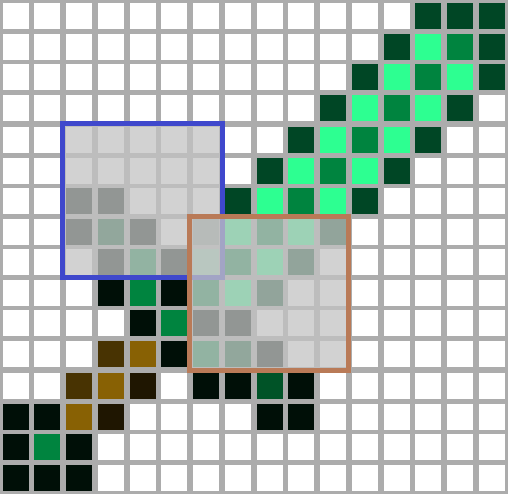
\includegraphics[width=4cm, height=4cm]{Graphics/diamon_sword_with_patches.png}
	\caption{Una imagen de $16 \times 16$ y dos parches de esta tomando $n = 25$.}
\end{figure}

\begin{definition}
	El p\'ixel o elemento central de un parche se encuentra en una posici\'on fija, dicha posici\'on debe ser la misma para todos los parches de una misma imagen.
\end{definition}

\begin{figure}[h]
	\centering
	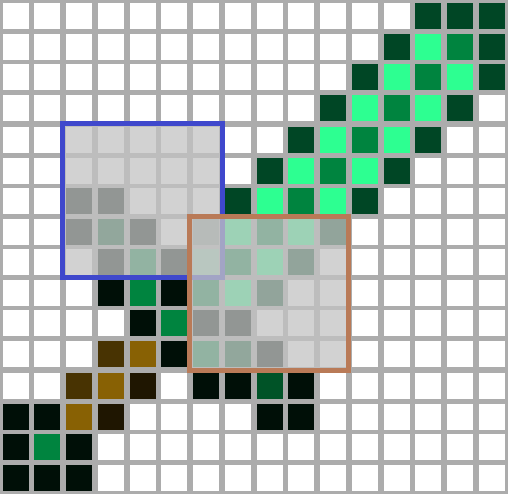
\includegraphics[width=4cm, height=4cm]{Graphics/diamon_sword_with_patches.png}
	\hspace{1cm}
	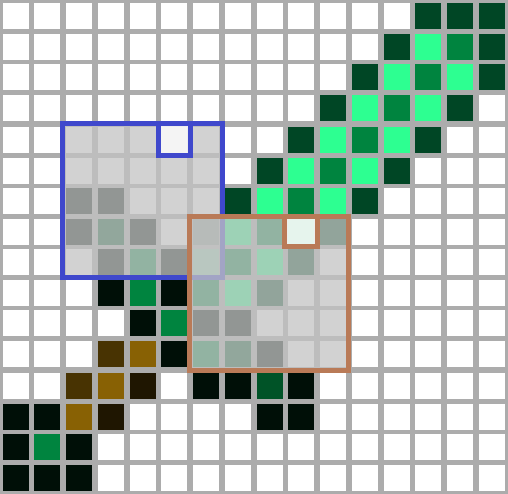
\includegraphics[width=4cm, height=4cm]{Graphics/diamon_sword_with_patches_and_centers.png}
	\caption{Parches con centro situado en la posici\'on $16$.}
\end{figure}

%	Ejemplo de definicion
%	
%	\begin{definition}
%  \label{EXPM}\cite{Golub96} Sea $A$ una matriz de $n\times n$ real o compleja. La exponencial de $A$ denotada por 
%  $ \me{A} $ o $\mathrm{exp}(A)$ es una matriz de $n\times n$ dada por la serie de potencias
%  \[\me{A}=\sum_{k=0}^{\infty}\frac{1}{k!}A^{k}.\]
%	\end{definition}

%	Ejemplo de teorema
%	\begin{theorem}\cite{IntroMatrix}
%	    La serie de matrices definida en~(\ref{EXPM-SERIE}) existe para toda matriz $A$ para $t$ fijo y
%	    para todo $t$ para $A$ fija. La serie converge uniformemente en cualquier regi\'on de t del plano complejo.
%	\end{theorem}

%	Ejemplo de ecuación
%	\begin{equation}
%	\me{tA}=I+tA+\frac{t^{2}A^{2}}{2!}+\cdots\label{EXPM-SERIE}
%	\end{equation}